% Chapter 1

\chapter{Progettazione} % Write in your own chapter title
\label{Chapter3} 

\section{Dimensionamento dei transistor}
\label{sec:dimensionamento}

In Tab. \ref{tab:dimensioniMos} le dimensioni ottenute per ciascun transitor.

\begin{table}[htb]
	\centering
	\begin{tabular}{c*{3}{c}}
		\toprule
		Id MOS & Rapporto d'aspetto & W($\mu$m) & L($\mu$m)\\
		\midrule
		1 & 30 & 3.24 & 0.12\\
		2 & 12 & 2.24 & 0.12\\
		\bottomrule
	\end{tabular}
	\caption{Tabella dimensioni MOS}
	\label{tab:dimensioniMos}
\end{table}

\section{Layout fisico}
\label{sec:layout}

In Fig. \ref{fig:layout} il layout finale del Full Adder TSPC.

\begin{figure}[hbt!]
	\centering
	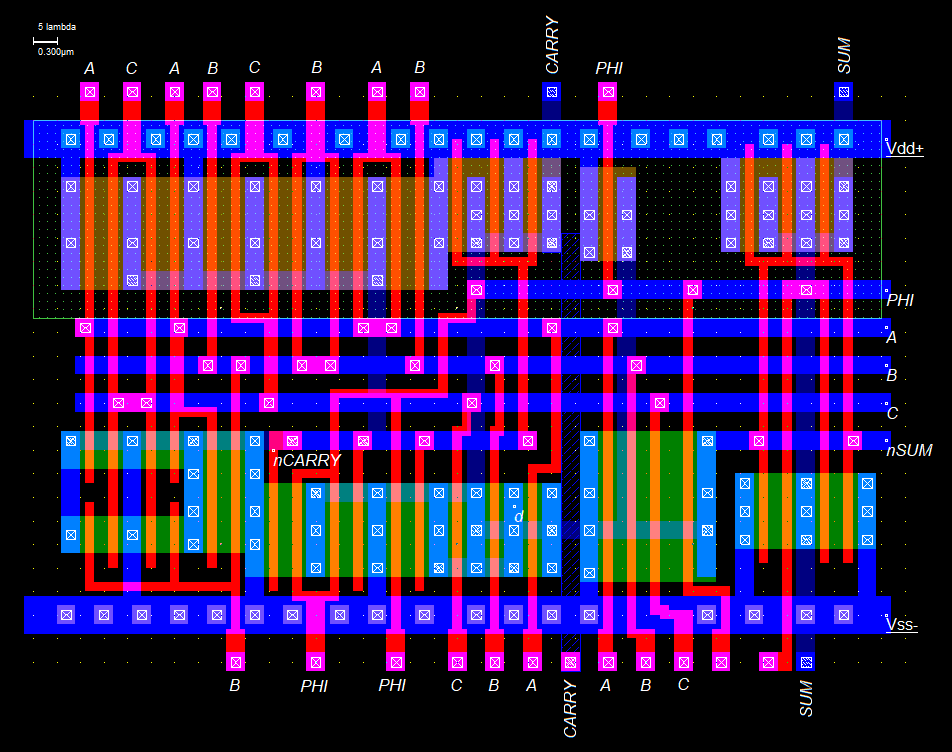
\includegraphics[width=1\textwidth]{figure/Msk_FullDesign.png}
	\caption{Layout finale.}
	\label{fig:layout}
\end{figure}





